\documentclass[../Matt_Gebert_Honours_Thesis.tex]{subfiles}

\begin{document}
% In \cref{chap:baregraphene} I will present the data and results from my measurements of the respective devices which will be placed on SiO$_2$. 

Graphene devices first need to have their transport properties measured in their pristine condition, prior to the application of thin oxides. Doing this will allow a comparison of the electrical transport properties before and after transfer, to see if there's any resulting enhancement. Here I analyse the resistance measurements taken for both graphene and CVD graphene. I will consider their dependence upon gate voltage and temperature.

\section{Resistance to resistivity}
The resistivity of a material is a core property that tells you it's behaviour in a bulk geometry. For 3D materials, resistivity is in the units of Ohms per meter. You can think about this single length proportionality coming from flowing charge through a cross section, but over some length. In 2D materials, resistivity is measured in Ohms, because there are only two dimensions, the length and the width of flat material. The partial form of the resistivity is listed in \cref{eqn:partial_resistivtiy}, where $w(L)$ is the width of the material as a function of Length.\\
\begin{minipage}{0.5\textwidth}
	\begin{align}
	\partial R = \frac{\rho}{w(L)}\partial L\label{eqn:partial_resistivtiy}
	\end{align}
	In most cases of devices we make, the geometry between probes can be described by either a rectangle or a trapezoid. There will be a resulting geometric factor that converts our resistance to resistivity.
	\begin{align}
	\rho = \mathcal{G} \times R
	\end{align}
\end{minipage}
\begin{minipage}{0.5\textwidth}
%	\begin{figure}
	\centering
	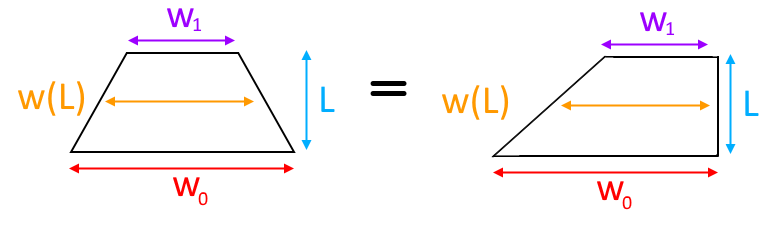
\includegraphics[width=0.9\textwidth]{chap4/geometry}
	\captionof{figure}{Two equivalent geometries of trapezoids.}
%	\end{figure}
\end{minipage}\\

For a rectangle, the width is independent of the length, and the geometric factor to convert resistance to resistivity becomes:
\begin{align}
\mathcal{G} = \frac{w}{L}
\end{align}
For a trapezoid, such as in  the width is linearly dependent upon length, and the geometric factor can be found as follows:
\begin{align}
	w(x) &= w_0 + \frac{x}{L}(w_1 - w_0)\\
	\frac{1}{\mathcal{G}} &= \int_{0}^{L}\frac{1}{w(x)}dx = \frac{l \left(\log\left[l w_0\right] - \log\left[l w_1\right]\right)}{w_0-w_1} = \frac{l \log\left[w_0/w_1\right]}{w_0-w_1}\\
	\implies \mathcal{G} &= \frac{w_0-w_1}{l \log\left[w_0 / w_1\right]}
\end{align}
In the limit w$_1\to$w$_2$, this result is consistent and returns to the rectangular case. I have included a few samples of which the geometric factor has been calculated:\\\newline
\begin{minipage}{0.5\textwidth}
	\centering
	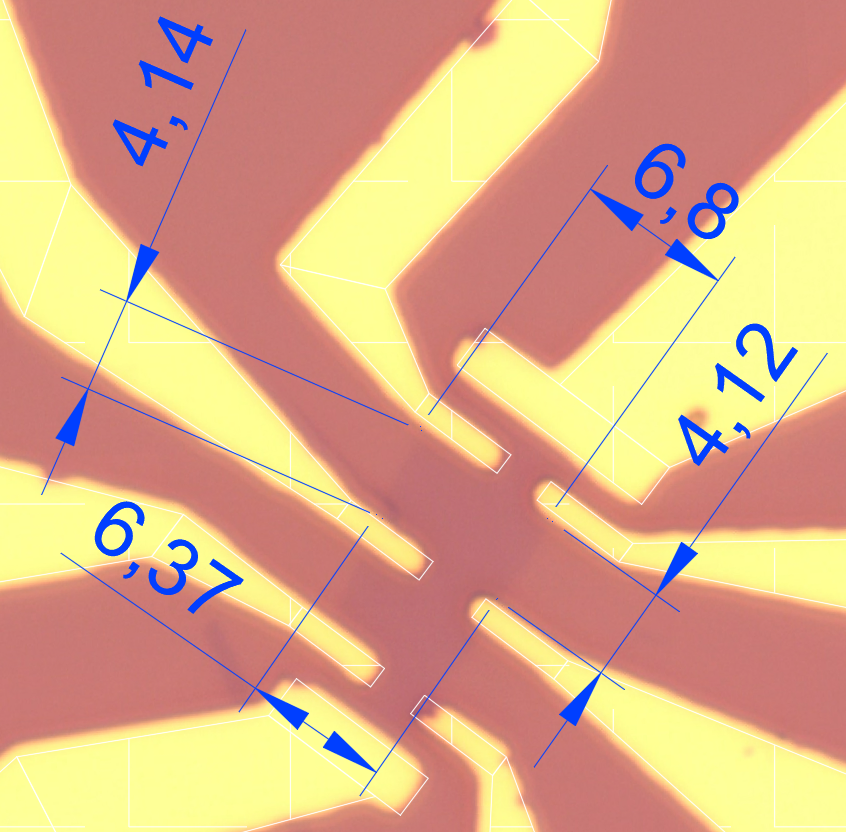
\includegraphics[width=0.5\textwidth]{chap4/exf6_geom}
	\captionof{figure}[EXF06 Geometry]{Geometry of exfoliated device 6 (EXF06). Units are in $\mu$m.}
\end{minipage}
\begin{minipage}{0.5\textwidth}
	\centering
	Using the graphene between the gold contacts on the upper half of the device, 
	\begin{align*}
		\mathcal{G} &= \left.\frac{w_0-w_1}{l \log\left[w_0 / w_1\right]}\right|_{L\to 4.12, w_0\to 6.37, w_1\to 6.8}\\ &= 1.59773
	\end{align*}
\end{minipage}\\\newline\hspace{0.5cm}
\begin{minipage}{0.5\textwidth}
	\centering
	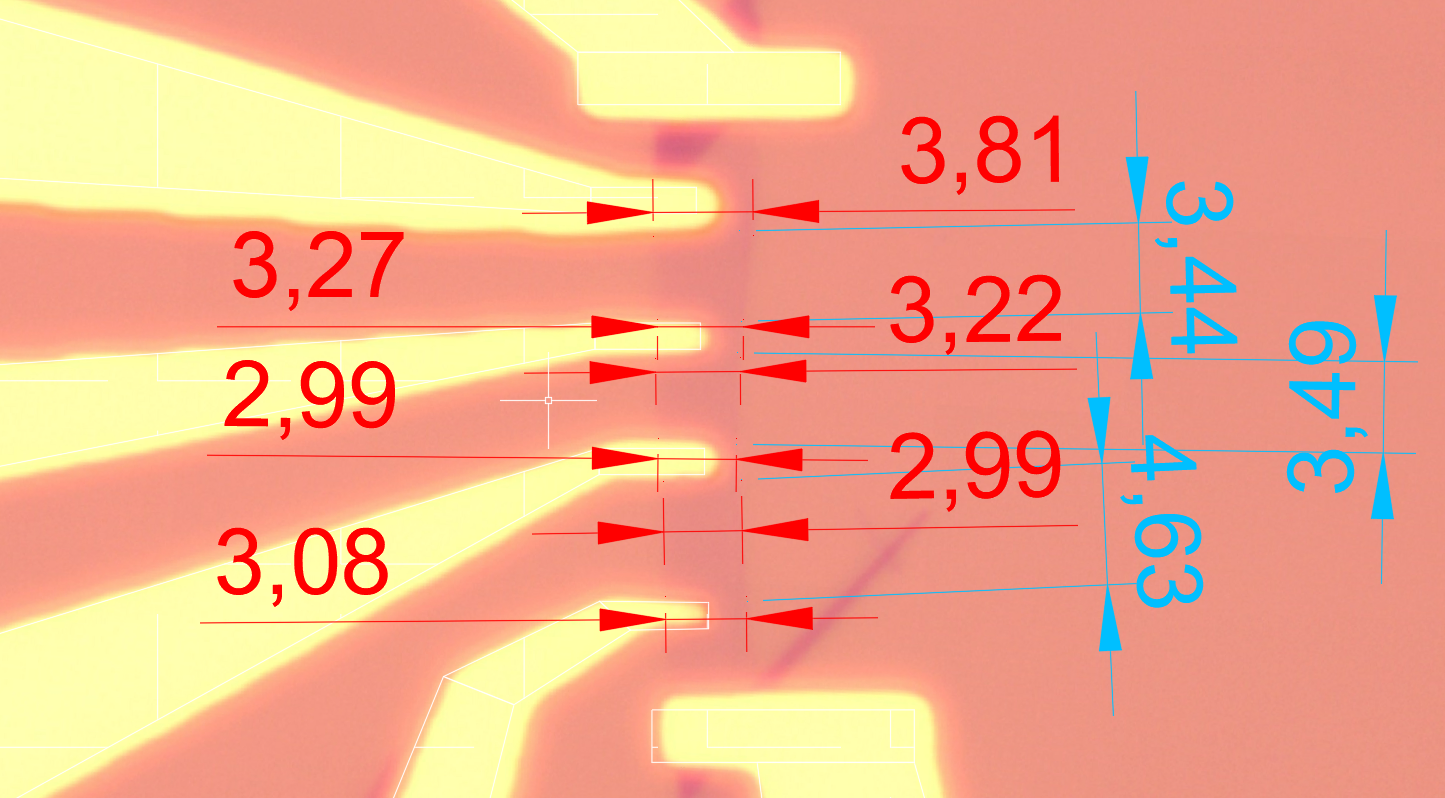
\includegraphics[width=0.9\textwidth]{chap4/exf4_geom}
	\captionof{figure}[EXF04 Geometry]{Geometry of exfoliated device 4 (EXF04). Units are in $\mu$m.}
\end{minipage}
\begin{minipage}{0.5\textwidth}
	\centering
	Geometric factors from top down: 
	\begin{align*}
	\mathcal{G}_A &= \mathcal{G}|_{L\to 3.44, w_0\to 3.81, w_1\to 3.27}\\ &= 1.02707\\
	\mathcal{G}_B &= \mathcal{G}|_{L\to 3.49, w_0\to 3.22, w_1\to 2.99}\\ &= 0.889278\\
	\mathcal{G}_C &= \mathcal{G}|_{L\to 4.63, w_0\to 2.99, w_1\to 3.08}\\ &= 0.65546\\
	\end{align*}
\end{minipage}\\\newline

This quantity is unclear for the transferred CVD graphene on top of gold pads because of the wide coverage across gold and short distances between current pads and voltage pads, however the relevant geometric quantity can still be found through the gate voltage dependent resistivity (Refer to \cref{sec:findinggeometricfactor}).

\section{Gate dependent conductivity}
After converting resistance measured to resistivity, I invert the resistivity to conductance. This now allows the fitting the gate voltage dependent conductivity (\cref{eqn:gate_dependent_conductivity}).
\begin{align}
\sigma = \sqrt{\left(N^{*} e \mu\right)^2 + \left(\rho_S + \frac{1}{N e \mu}\right)^{-2}} \label{eqn:gate_dependent_conductivity}
\end{align}
Here $N^{*}$ (also written as $\mathcal{N}$) is the `residual carrier density'  ($m^{-2}$) \cite{adam_self-consistent_2007}, $N$ is the carrier density ($m^{-2}$), e is the elementary charge, $\mu$ is the mobility ($m^2/Vs$) and $\rho_S$ is a resistivity parameter that affects the curvature of of the gate voltage dependent conductivity, particularly in the high voltage limits, but it's origins are unclear.
The carrier density $N$ is calculated by considering the accumulated charge at the gate. This amount can be calculated for each device, by considering the capacitance of 285nm \silicondioxide{} and the difference in gate voltage from the Dirac point.
\begin{align}
	N(V_G) &= \frac{C_g}{e} \left|V_{\text{Dirac}}-V_G\right|\\
	C_g &= \epsilon \frac{A}{d} = 3.8 \times 8.85 \times 10^{-12} \frac{1}{285\times 10^{-9}} \approx 1.2 \times 10^{-4}
\end{align}

In using this fitting function, I only apply the fit to one side of the Vg vs $\rho$ curve's data at a time. This means that the mobility parameter $\mu$ is treated separately for hole and electron like conduction. 

Fitting was performed on conductivity data, so that parameter fits were sensitive to curvature far from the Dirac point. Unfortunately, this also meant that sensitivity to the Dirac point was lacking during fitting. As a result, I added extra weighting to data near the Dirac point, to ensure the charge impurity parameter $\mathcal{N}$ enforced a good match at the minimum conductivity turning point. This action I took is justified, because if the impurity parameter is not properly fitted, then linked parameters such as the mobility will be incorrectly determined. An example fit for EXF06 is shown in \cref{fig:exf06_78K_VgR}, the same parameters plotted over resistivity and conductivity:
\begin{figure}[H]
	\centering
	\begin{subfigure}{0.4\textwidth}
		\centering
		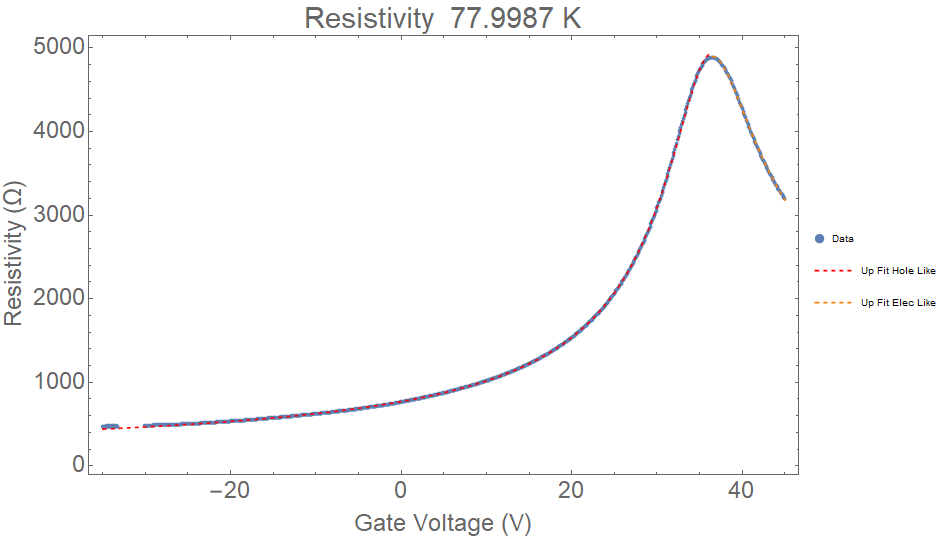
\includegraphics[width=\textwidth]{chap4/exf06/EXF006_Asym_Res_vs_Vg_at_Temp_78K}
%		"chap4/exf06/EXF006_Asym_Res_vs_Vg_at_Temp_78.K.png"
		\caption{Resistivity fit}
	\end{subfigure}
	\begin{subfigure}{0.4\textwidth}
		\centering
		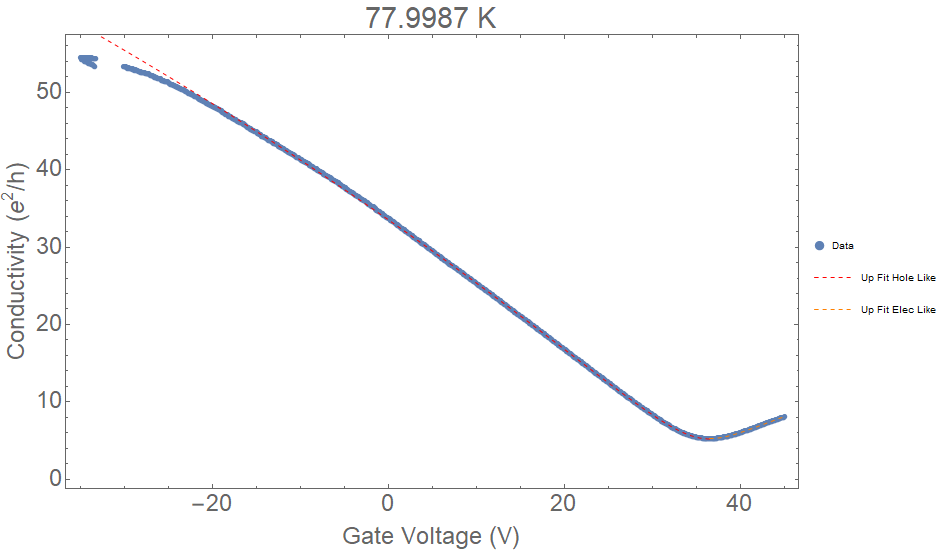
\includegraphics[width=\textwidth]{chap4/exf06/EXF006_Asym_Cond_vs_Vg_at_Temp_78K}
		\caption{Conductivity fit}
	\end{subfigure}
	\begin{subfigure}{0.16\textwidth}
		\centering
		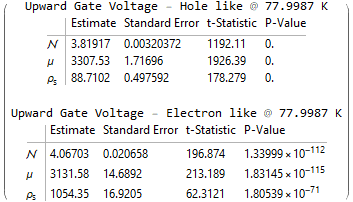
\includegraphics[width=\textwidth]{chap4/exf06/EXF006_Asym_Param_Fit_78K}
		\caption{Fit parameters}
	\end{subfigure}
	\caption[Gate dependent transport of EXF06]{Gate dependent transport of EXF06 at 78K. \\Note parameter units are: mobility $\mu$ in cm$^2$/Vs, $\mathcal{N}$ in $\times 10^{15}$/m$^2$, and $\rho_S$ in  $\Omega$}\label{fig:exf06_78K_VgR}
\end{figure}

Here the conductivity has been scaled in terms of the conductivity quantum, $e^2/h$ .Further fits for devices at different temperatures can be found in appendix \ref{app:fits}.

\subsection{Finding the geometric factor of CVD graphene}\label{sec:findinggeometricfactor}
I previously mentioned the issue with finding a geometric factor for CVD graphene. It turns out that from finding the residual carrier density parameter $\mathcal{N}$, we can scale our data to match the correct theoretical mobility $\mu$ predicted for that particular $\mathcal{N}$. The theoretical data we use to find the matching mobility is provided in appendix \ref{app:transport_theoretical}.

A new fit doesn't change the determined $\mathcal{N}$ value, because the mobility $\mu$ is a parameter that scales the minimum conductivity point along with the conal regions $\to$ $\mathcal{N}$ is independent of scaling. 

My method of determining the geometric value is as follows:
\begin{enumerate}
	\itemsep0em
	\item Find minimum conductivity value
	\item Scale conductivity data such that minimum conductivity is $\approx$4 ($e^2/h$). This is a ballpark figure for most graphene samples\cite{tan_measurement_2007}, and will allow us to get close to the desired mobility $\mu$ and residual carrier density $\mathcal{N}$. 
	\item Fit the conductivity data to \cref{eqn:gate_dependent_conductivity} to find $\mathcal{N}$ and $\mathcal{\rho_S}$. 
	\label{enum:fit}
	\item Refer to the theoretical data in appendix \ref{app:transport_theoretical} to find the corresponding mobility $\mu_0$ for the particular $\mathcal{N}$.
	\item Scale conductivity by $\lambda$ such that $\left.\sigma\right|_{\mathcal{N},\rho_S,\mu\to\mu_0} \times \lambda = 4 e^2/h$
	\item Repeat step 3 to make sure $\mu$ and $\mathcal{N}$ match up.
	\item Calculate geometric factor $\frac{1}{\mathcal{G}} = \frac{\text{Scaled minimum conductivity}}{\text{Original minimum conductivity}}$
\end{enumerate}

To check the validity of this method, I compare the geometric factors calculated above for EXF06 to the numerically determined values.%\\\newline %TODO: EXF04 if time.

%\begin{minipage}{0.5\textwidth}
	\paragraph{EXF06}
	Raw data minimum conductivity was originally 8.5061 ($e^2/h$) at 88K. All conductivity values were divided by 2.1265 to bring the minimum back to 4. Fitting was then done to find the residual carrier density $\mathcal{N}$, seen in \cref{fig:geomfit1}.
	\begin{figure}[H]
		\begin{subfigure}[b]{0.6\textwidth}
			\centering
			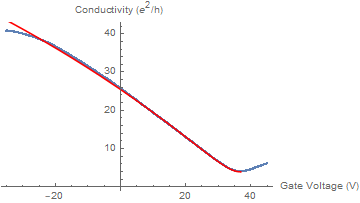
\includegraphics[width=\textwidth]{chap4/exf06/geom_fit1}
			\caption{First fit}
		\end{subfigure}
		\begin{subfigure}[b]{0.4\textwidth}
			\centering
			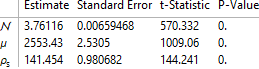
\includegraphics[width=0.7\textwidth]{chap4/exf06/geom_fit1_params}
			\captionof{figure}{First fit params}\label{fig:geomfit1params}		
		\end{subfigure}
		\caption[Geometric factor fitting to find $\mathcal{N}$]{First fit to find $\mathcal{N}$}\label{fig:geomfit1}
	\end{figure}
	Finding the value $N^{*} = 3.76\times10^{15}$ in appendix \ref{app:transport_theoretical}, we interpolate the corresponding mobility to 0.3460 m$^2$/Vs. Then finding the scaling factor for the conductivity:
	\begin{align}
		\lambda \times \sigma\left[\rho_{s}\to 141, \mu\to 0.3460, \mathcal{N}\to 3.76\times 10^{15}\right] &= 4\\
		\implies \lambda &= 0.743448
	\end{align}
	The conductivity is then scaled by the reciprocal of this value, so that the minimum conductivity moves from 4, and allows the appropriate scaling of $\mu$ to match $\mathcal{N}$. The minimum conductivity is now scaled to 5.38034 ($e^2/h$).
	
	Performing a second fit to check the new value,
	\begin{table}[H]
		\centering
		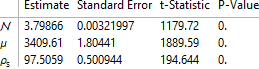
\includegraphics[width=0.4\textwidth]{chap4/exf06/geom_fit2_params}
		\caption[Geometric factor fitting to find $\mu$]{Second fit to confirm $\mu$ scaling}\label{fig:geomfit2}
	\end{table}
	The mobility is now $3409.61$ cm$^2$/Vs which is very close to 3448.28 cm$^2$/Vs (the tabled value corresponding to $\mathcal{N}=3.79353\times10^{15}$/m$^2$). I could perform a few more iterations to get the mobility even more closer to the theoretical, but seeming I am interpolating non-linear data  between rows, I deemed this to be unnecessary, particularly given the final result.

	Now finding the relative factor between the original minimum conductivity and the scaled minimum conductivity:
	\begin{align}
		\frac{1}{\mathcal{G}} &= \frac{5.38034}{8.5061} = 0.632524\\
		\implies \mathcal{G} &= 1.58097
	\end{align}
	This is almost exactly a 1\% difference from our image found geometric value of $\mathcal{G} = 1.59773$, which shows the reliability of this method. 
	It's noteworthy that finding the geometric value from images will have a degree of uncertainty ($\approx$10\%) in the width and length values used, due to the scaling of images and placement of dimension markers.

	\paragraph{CVD01}
	Performing the same analysis in our dataset for CVD graphene, I find the minimum conductivity scales from 47.7959 ($e^2/h$) to 4.3794 ($e^2/h$), when the mobility $\mu$ and residual carrier density $\mathcal{N}$ converge on 0.157402 m$^2$/Vs and 6.67275 $\times10^{15}$/m$^2$ respectively (rows 63 \& 64 of appendix \ref{app:transport_theoretical}). This results in a geometric factor of $\mathcal{G} 10.7959$.

	Considering the visual geometry of our CVD graphene in \cref{fig:cvd_sample}, this is likely a reasonable geometric factor, given for a rectangular case $\mathcal{G}$ goes as W/L. In the figure, the majority of the current probably flows through the gold probes rather than through the bulk graphene, and considering the width to length ratio between those probes, I'd suggest it's approximately a factor of 10.
	\begin{figure}[H]
		\centering
		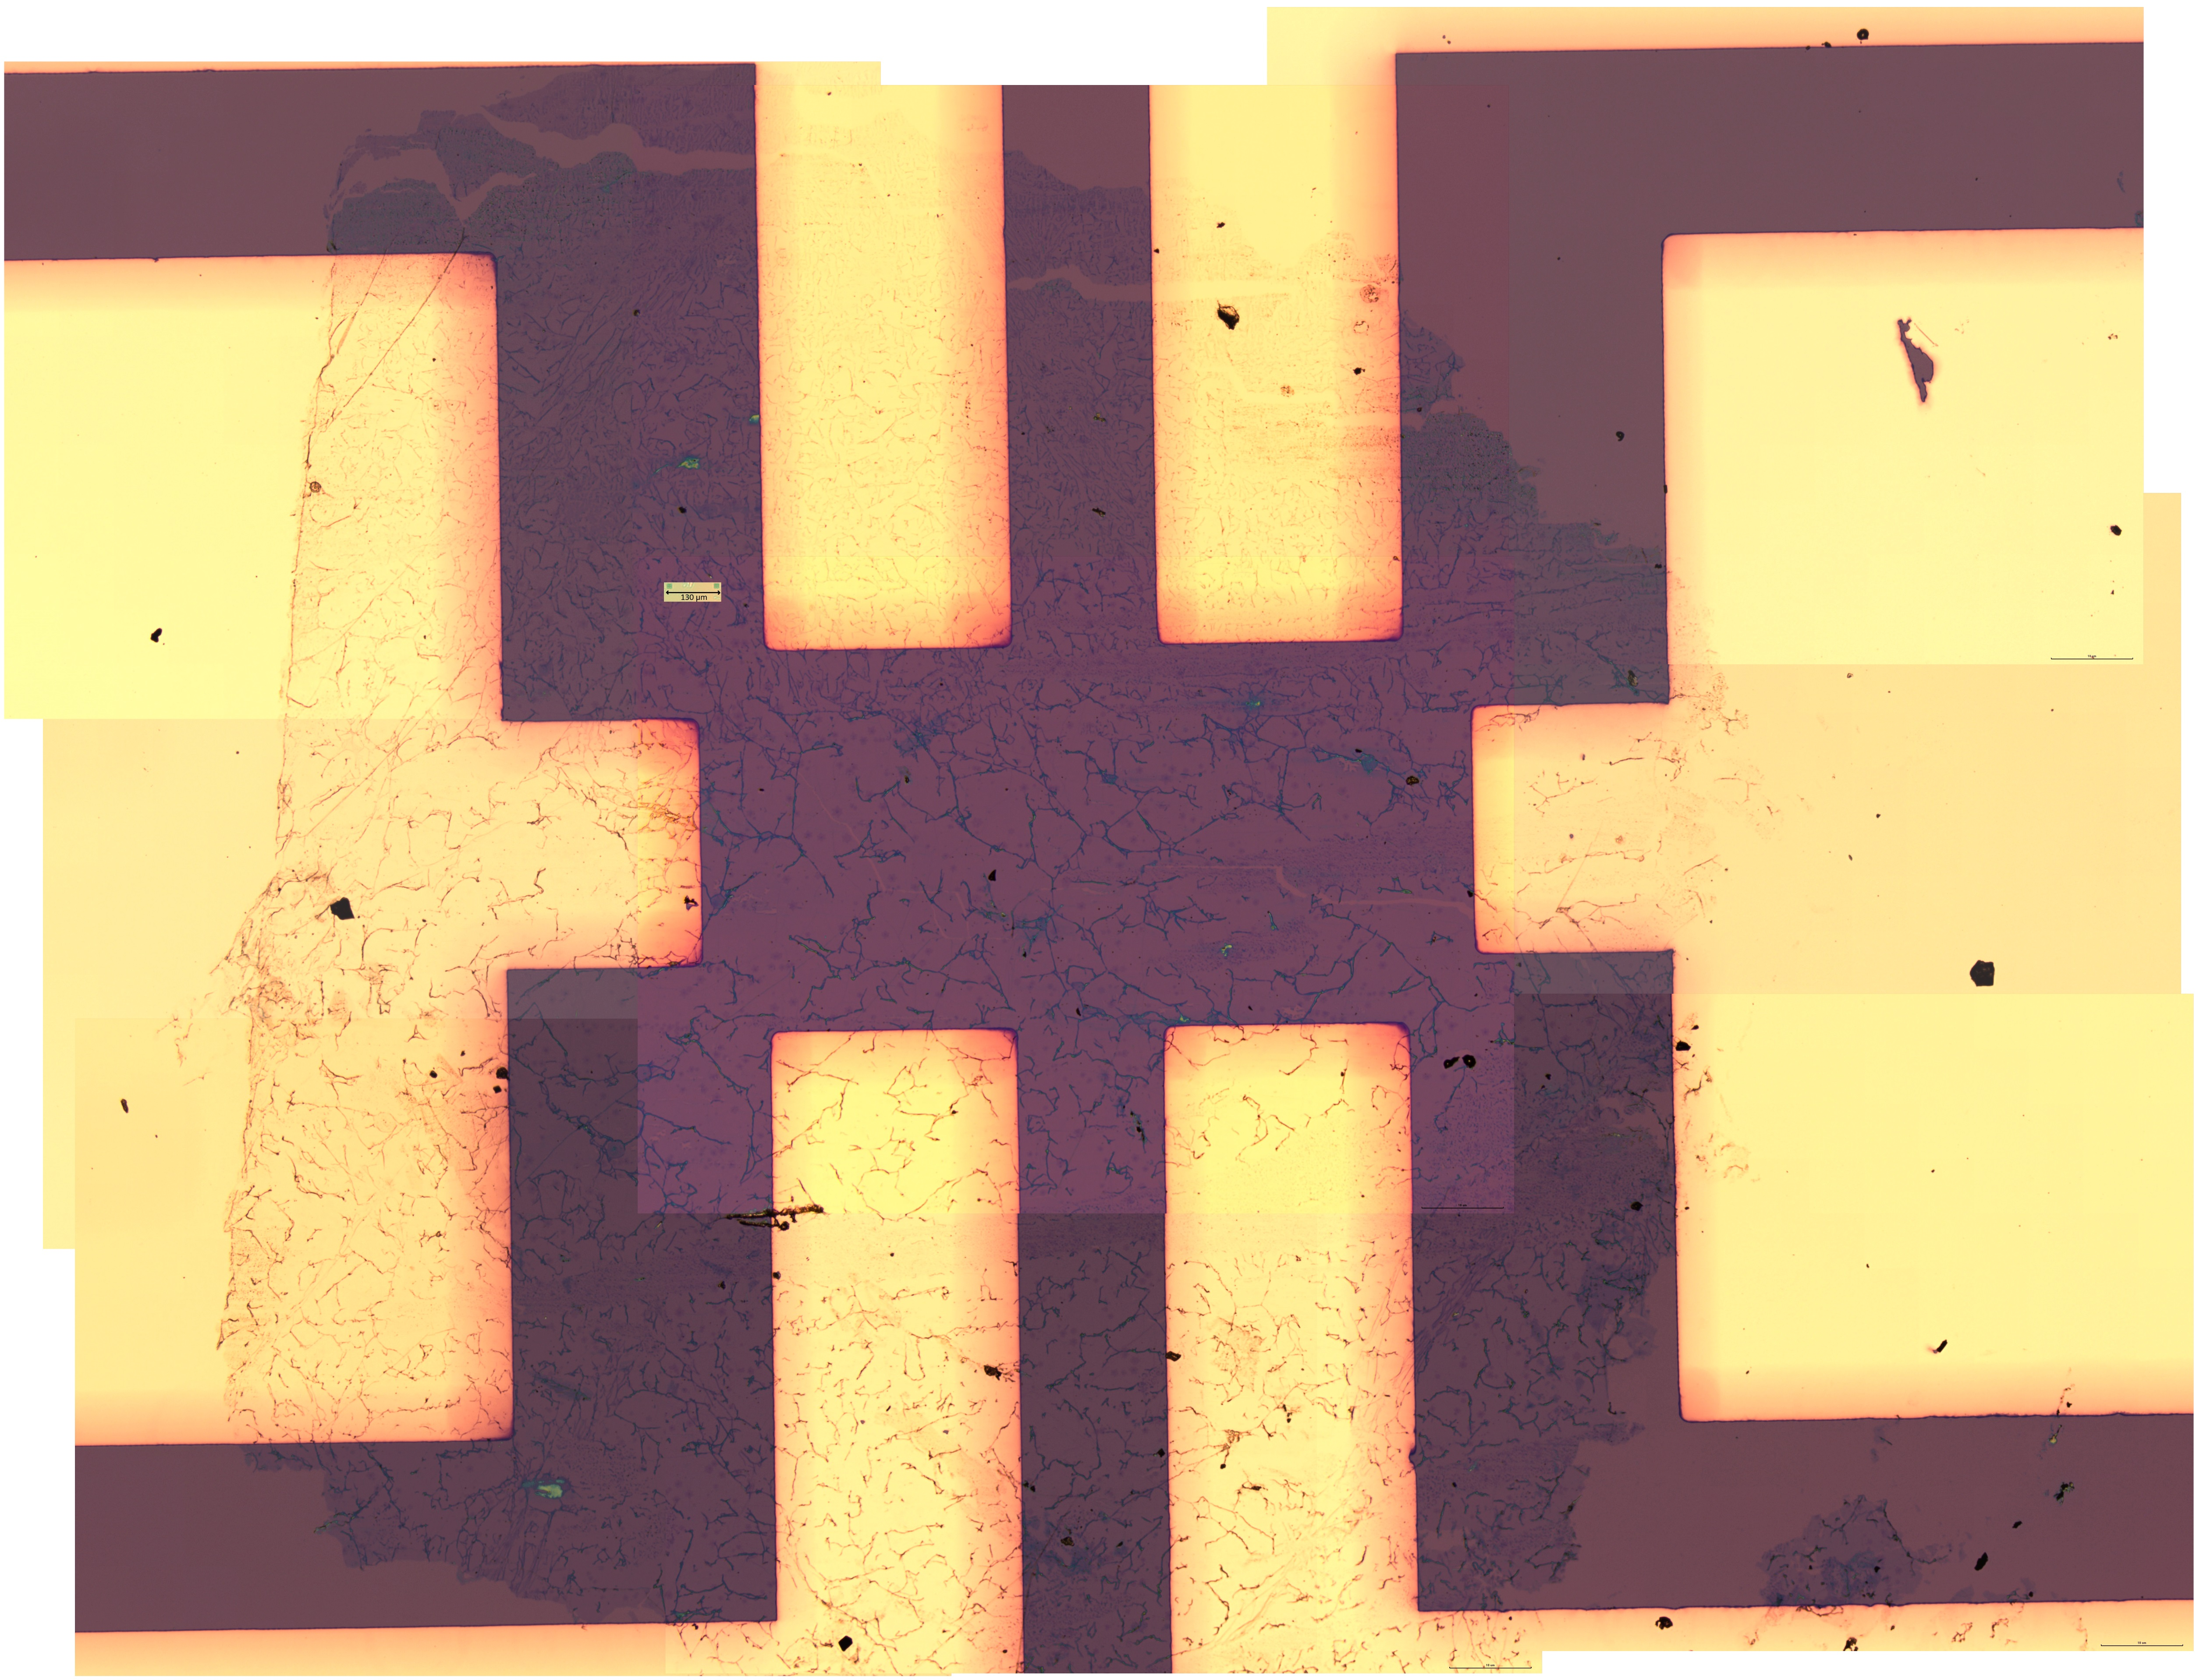
\includegraphics[width=0.4\textwidth]{chap2/cvd_graphene}
		\caption[Device CVD01]{Chemical vapour deposition device CVD01}\label{fig:cvd_sample}
	\end{figure}

\section{Temperature \& gate dependent conductivity}
For two devices, CVD01 and EXF06 I was able to capture a reasonable spread of temperature data to analyse the phonon contributions to graphene's transport properties. The qualitative change in their gate voltage - conductivity (VgC) curves are shown below.

\begin{figure}[H]
	\begin{subfigure}[b]{0.5\textwidth}
		\centering
		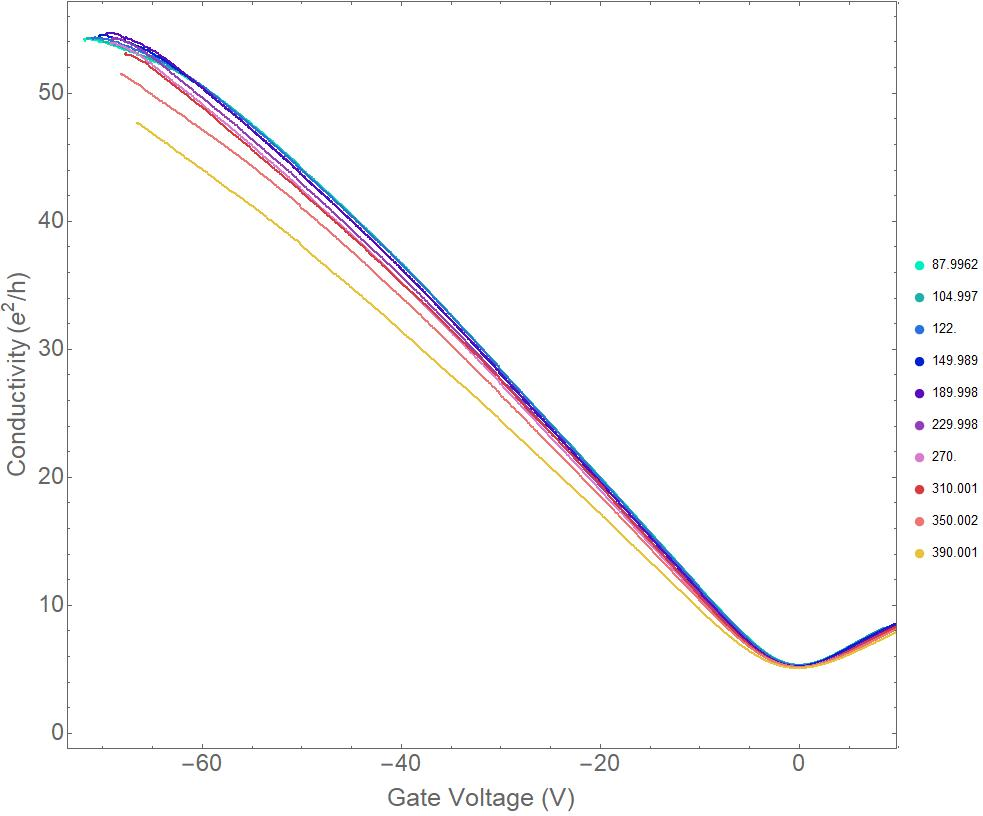
\includegraphics[width=\textwidth]{chap4/exf06/EXF006_Cond_vs_T_plot_centred}
		\caption{EXF06}
	\end{subfigure}
	\begin{subfigure}[b]{0.5\textwidth}
		\centering
		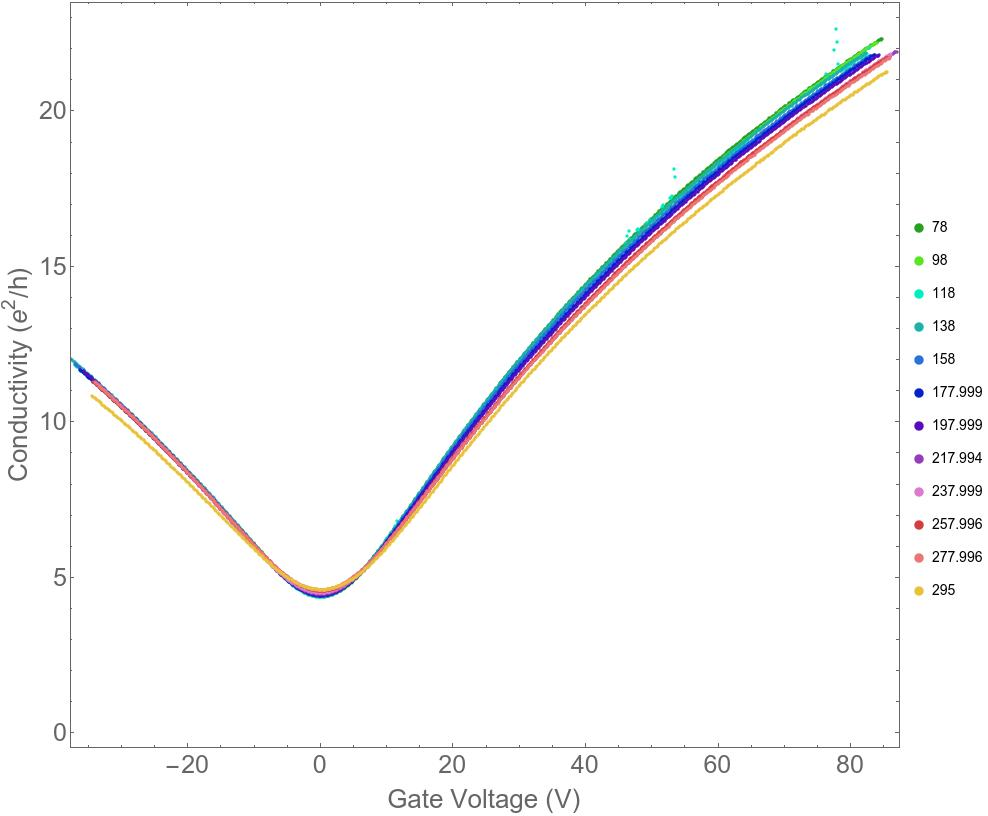
\includegraphics[width=\textwidth]{chap4/cvd01/CVD001_Cond_vs_T_plot}
		\caption{CVD01}
	\end{subfigure}
	\caption[Changes in gate-voltage conductivity with temperature]{Temperature dependence of VgC curves. Here the gate voltages have been shifted so that the Dirac point of each temperature data run is found at 0V.}
\end{figure}

It is clear that in both CVD01 and EXF06 that as temperature increases, the resistivity of graphene increases, as the slope of the conductivity clearly drops off in higher carrier density.

\subsection{$V_G$ R mobility}

Having fitted \cref{eqn:gate_dependent_conductivity} for each temperature, the fitted mobility parameter can be plotted across temperature. Strictly, $\mu(T,V_g) = \frac{\sigma(V_g,T)}{n(V_g) e }$ such that the mobility should be a function of gate voltage and temperature (see below), however I have found temperature dependent mobility which doesn't consider gate dependence. This is a relevant measure, but not concrete.
\begin{figure}[H]
	\centering
	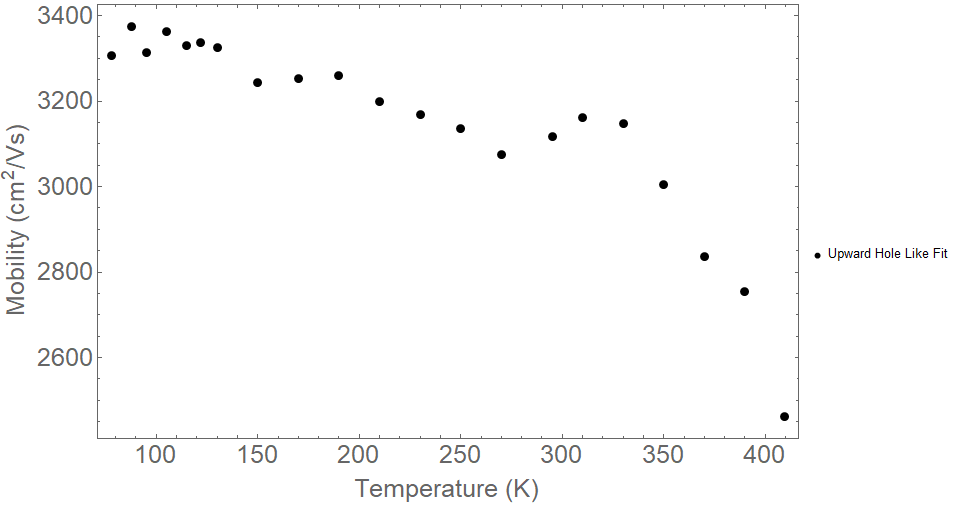
\includegraphics[width=0.7\textwidth]{chap4/exf06/EXF006_asym_mobility_vs_T}
	\caption{Gate voltage  vs resistivity temperature dependent mobility for EXF06}\label{fig:temp_mobility}
\end{figure}

At low temperature  ($\leq 130K$) LA phonons in graphene are expected to weakly dominate scattering, but at higher temperature remote phonon scattering from \silicondioxide{} is expected to dominate \cite{chen_intrinsic_2008}. This is clear in \cref{fig:temp_mobility}, particularly with the steep decent in mobility after 300K.

\subsection{Temperature dependent conductivity}
As described above, a more comprehensive analysis of the conductivity is required to really determine the mobility behaviour. I fit the conductivity across gate voltage and temperature, and show the remote phonon contribution to temperature and gate dependent conductivity.
\begin{align}
\rho[V_g,T] = \rho_0[V_g] + \rho_A[T] + \rho_B[Vg,T] \label{eqn:temp_resistivity}
\end{align}
To investigate the contribution of phonons (both longitudinal acoustic and remote polar) to resistivity using the temperature spread of the data taken for devices, my fitting function (\cref{eqn:temp_resistivity}) comprises of three components. $\rho_0$ is the intrinsic gate dependent resistivity found near 0K (we have to allow a free parameter $R_0$ due to not having a measurement near absolute zero), $\rho_A$ is the longitudinal acoustic phonons found within graphene which scales linearly with temperature, and $\rho_B$ is the contribution from remote polar phonons found in \silicondioxide{} affected by both the gating voltage (affecting the polarity) and the temperature (vibrational excitations).
\begin{align}
\rho_A[T] &= \left(\frac{h}{e^2}\right) \frac{\pi2 Da^2 k_B T}{2 h^2 \rho_S V_s^2 V_F^2}\label{eqn:acoustic_phonon}\\
\rho_B[V_G,T]&= B \frac{h}{e^2} V_G^{-\alpha_1} \left(\begin{aligned}
&\frac{1}{\exp\left[(0.059\text{ eV})/k_B T\right]-1}\\ &\hspace{2cm}+\frac{6.5}{\exp\left[(0.115\text{ eV})/k_B T\right]-1}
\end{aligned}\right)\label{eqn:remote_phonon}
\end{align}
For \cref{eqn:acoustic_phonon}, $k_B$ is the Boltzmann constant, $\rho_s$ is the 2D mass density of graphene, $v_F$ is the Fermi velocity, $v_s$ is the velocity of sound and $D_A$ is a fitted parameter, the deformation potential.
\cref{eqn:remote_phonon} is a combination of two surface phonons in \silicondioxide{}, given by Bose-Einstein distributions \cite{chen_intrinsic_2008}. These distributions come from the optical phonon energies in \silicondioxide{}, at 59 meV and 155 meV \cite{fratini_substrate-limited_2008}.
\subsubsection{EXF06 - Exfoliated graphene}
I used three different fits to observe the presence of these phonons in graphene. 
The fit parameters in \cref{fig:phonon_fit_params} correspond to the curves in \cref{fig:exf_temp_gate}.
\begin{table}[H]
	\begin{subfigure}[b]{0.3\textwidth}
		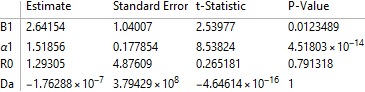
\includegraphics[width=\textwidth]{chap4/exf06/phonons/temp270params}
		\caption{$T < 270 ^\circ K$}\label{fig:phononA270}
	\end{subfigure}\hspace{0.03\textwidth}
	\begin{subfigure}[b]{0.3\textwidth}
		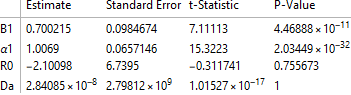
\includegraphics[width=\textwidth]{chap4/exf06/phonons/tempSampledparams}
		\caption{$T < 270 ^\circ K, T > 370 ^\circ K$}\label{fig:phononASamp}
	\end{subfigure}\hspace{0.03\textwidth}
	\begin{subfigure}[b]{0.3\textwidth}
		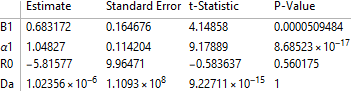
\includegraphics[width=\textwidth]{chap4/exf06/phonons/tempFullparams}
		\caption{$70 ^\circ K < T < 410 ^\circ K$}\label{fig:phononAFull}
	\end{subfigure}
	\caption{Phonon fit parameters}\label{fig:phonon_fit_params}
\end{table}

Our results for the remote phonon contributions are quite close to that of Chen \etal{.}\cite{chen_intrinsic_2008} when I include the upper data (\cref{fig:phononASamp,fig:phononAFull}), with $\alpha_1$ \& B1 parameters $\approx$ 1.02 \& 0.7 respectively, matching 1.04 and 0.6 from Chen \etal{.} \cite{chen_intrinsic_2008}, showing that the remote phonon contributions can reliably be detected in our devices.

\begin{figure}[H]
	\begin{subfigure}[b]{0.45\textwidth}
		\centering
		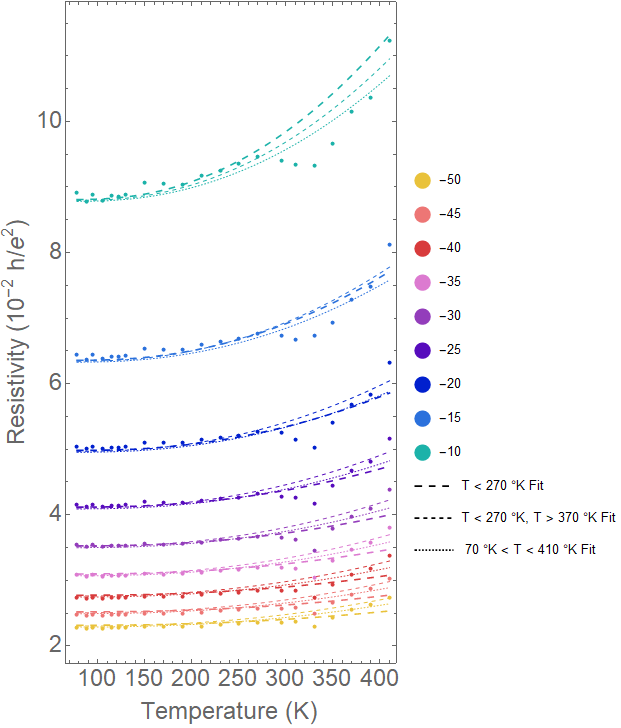
\includegraphics[width=\textwidth]{chap4/exf06/phonons/EXF006_Res_vs_T_upward}
		\caption[EXF06 temperature dependent conductivity]{Gate and temperature dependent conductivity of EXF06.}\label{fig:exf_temp_gate}
	\end{subfigure}\hspace{0.05\textwidth}
	\begin{subfigure}[b]{0.45\textwidth}
		\centering
		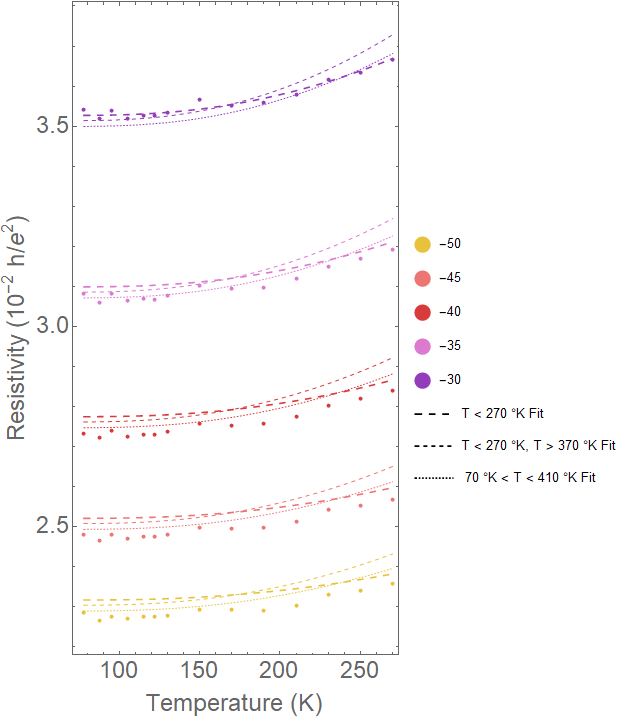
\includegraphics[width=\textwidth]{chap4/exf06/phonons/EXF006_Res_vs_T_upward270}
		\caption[EXF06 temperature dependent conductivity]{Gate and temperature dependent conductivity of EXF06.}\label{fig:exf_temp_gate_zoom}
	\end{subfigure}
	\caption[Gate and temperature dependence of resistivity for EXF06]{Gate and temperature dependence of resistivity for EXF06. 3 fits have been conducted over different domains due to the bump that occurs at about 330 $^\circ$K}
\end{figure}

However, the fits for the longitudinal acoustic phonons are very poor, with the $D_a$ parameter not fitting in any of the examples. To attempt to fit to solely the longitudinal acoustic phonon contribution, I took data between 78 $^\circ$K and 130 $^\circ$K, reflecting the linear region of the acoustic phonon contribution in Chen \etal{}, and removed the remote phonon contribution $\rho_B$ to the fitting function. 
I also tried adding further freedom in the initial resistance, by adding a free parameter for every gate voltage, in order to observe the longitudinal acoustic phonon contribution. 

\begin{figure}[H]
	\begin{subfigure}[t]{0.5\textwidth}
		\centering
		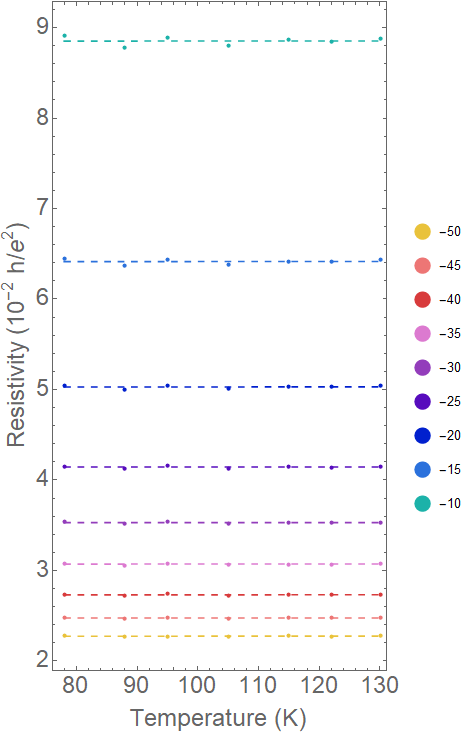
\includegraphics[width=0.5\textwidth]{chap4/exf06/phonons/LAphonons}
		\caption{LA phonon fitting at low temperature}
	\end{subfigure}
	\begin{subfigure}[t]{0.5\textwidth}
		\centering
		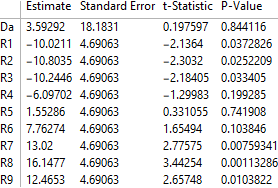
\includegraphics[width=0.5\textwidth]{chap4/exf06/phonons/LAphononsParams}
		\caption{LA phonon parameters}
	\end{subfigure}
	\caption[EXF06 LA phonon fitting]{Fitting of EXF06 to LA phonons in low temperature data}\label{fig:exf06_laphonon}
\end{figure}

\Cref{fig:exf06_laphonon} has given the first successful fit to a LA phonon contribution, however the $D_a$ parameter is far from the theoretical prediction seen in Chen \etal{.}\cite{chen_intrinsic_2008} at 18 eV, significantly reducing any contribution. The data is visually unconvincing in linear gradient at this scale. 
I have also attempted to fit the full resistivity contribution again using the extra freedom in the offset resistance parameters in 

\begin{table}[H]
	\begin{subfigure}[b]{0.3\textwidth}
		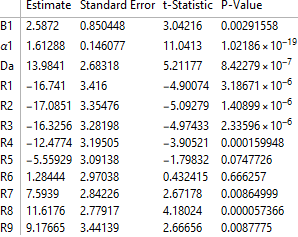
\includegraphics[width=\textwidth]{chap4/exf06/phonons/temp270paramsR}
		\caption{$T < 270 ^\circ K$}\label{fig:phononB270}
	\end{subfigure}\hspace{0.03\textwidth}
	\begin{subfigure}[b]{0.3\textwidth}
		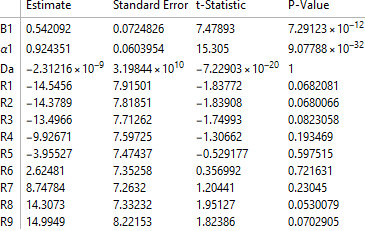
\includegraphics[width=\textwidth]{chap4/exf06/phonons/tempSampledparamsR}
		\caption{$T < 270 ^\circ K, T > 370 ^\circ K$}\label{fig:phononBSamp}
	\end{subfigure}\hspace{0.03\textwidth}
	\begin{subfigure}[b]{0.3\textwidth}
		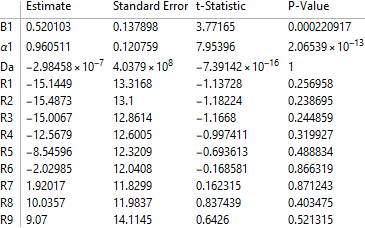
\includegraphics[width=\textwidth]{chap4/exf06/phonons/tempFullparamsR}
		\caption{$70 ^\circ K < T < 410 ^\circ K$}\label{fig:phononBFull}
	\end{subfigure}
	\caption[Gate and temperature dependence of resistivity fit parameters for EXF06 with R flexibility]{Gate and temperature dependence of resistivity fit parameters for EXF06 but with each gate voltage having a scalar-resistance degree of freedom.} \label{fig:exf_temp_gateRparams}
\end{table}

\begin{figure}[H]
	\begin{subfigure}[b]{0.5\textwidth}
		\centering
		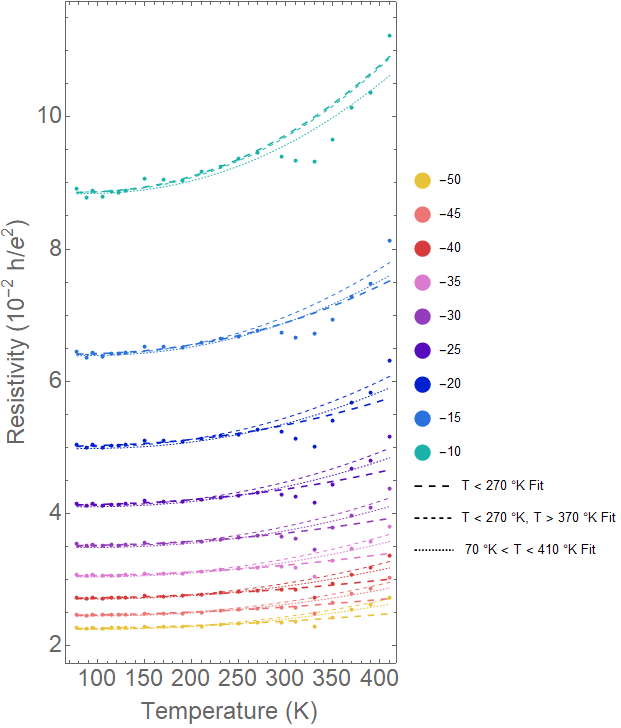
\includegraphics[width=0.7\textwidth]{chap4/exf06/phonons/EXF006_Res_vs_T_upwardR}
		\caption[EXF06 temperature dependent conductivity]{Gate and temperature dependent conductivity of EXF06.}\label{fig:exf_temp_gateR}
	\end{subfigure}
	\begin{subfigure}[b]{0.5\textwidth}
		\centering
		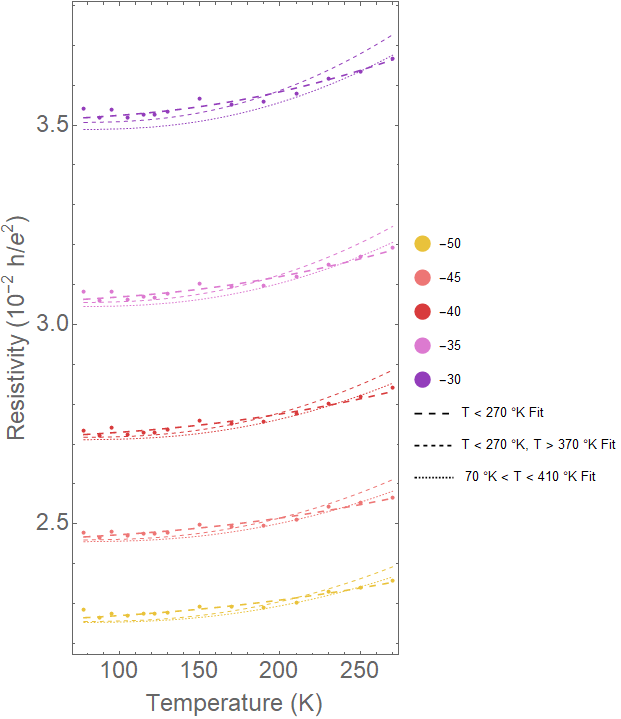
\includegraphics[width=0.7\textwidth]{chap4/exf06/phonons/EXF006_Res_vs_T_upward270R}
		\caption[EXF06 temperature dependent conductivity]{Gate and temperature dependent conductivity of EXF06.}\label{fig:exf_temp_gate_zoomR}
	\end{subfigure}
	\caption[Gate and temperature dependence of resistivity for EXF06 with R flexibility]{Gate and temperature dependence of resistivity for EXF06. 3 fits have been conducted over different domains due to the bump that occurs at about 330 $^\circ$K. Each gate voltage has a scalar resistance degree of freedom.}
\end{figure}

Lastly, the fits of \cref{fig:exf_temp_gateR} and \cref{fig:exf_temp_gateRparams} successfully fit to a reasonable LA phonon contribution ($D_a\to 13.9\pm 2.7$ eV) in the subset of data under the temperature of 270 $^\circ$K. This is a little more convincing, but likely just fitting to the remote phonon contribution past 130 $^\circ$K. 


There are a few good possible reasons as to why EXF06 did not see clearly see the longitudinal acoustic phonons from graphene. Firstly, there is a big kink in the temperature dependent curve at all gate voltages. I suspect that this was due to the fact that this sample was cooled to about 150 $^\circ$K before the turbo pump was activated. It is highly likely that adsorbates condensed on the surface of the graphene that we were measuring, affecting the amount of trapped charges and impurities and increasing scattering on graphene. It becomes clear then that if this condensed material evaporates around room temperature, the conductivity would increase as seen, before the remote phonon contribution outscales any gains made by evaporation of absorbates. It is unclear when the evaporation begins however, and this could completely mask evidence of longitudinal acoustic phonons.

Additionally to the point, the data acquired by Chen \etal is taken in ultra high vacuum (UHV) at about $10^{-10}$ mBar which would provide an extremely clean environment, compared to our turbo pump at $10^{-5}$ mBar.

Secondly, the gated mobility of this devices was around 0.33 m$^2$/Vs, which is comparably low to other exfoliated devices with around 1.6 m$^2$/Vs. As a result, the gate-voltage dependent resistivity isn't as sharp. Sharpness is desired to add spread in temperature measurements, where small phonon contributions might be more easily identified. This isn't as significant as the effect of absorbates, but still relevant.

Finally, we can use the parameter set in \cref{fig:phononASamp} to determine the mobility in \cref{eqn:mobility}.
\begin{align}
	\mu\left[V_g,T\right] = \frac{\sigma\left[V_g,T\right]}{N\left[V_g\right]\times e}\label{eqn:mobility}
\end{align}
Plotting for a few different gate voltages in \cref{fig:exf06_mobility}, there's general consistency and agreement between the gate-voltage mobility and the full temperature-gate-voltage dependent mobility:
\begin{figure}[H]
	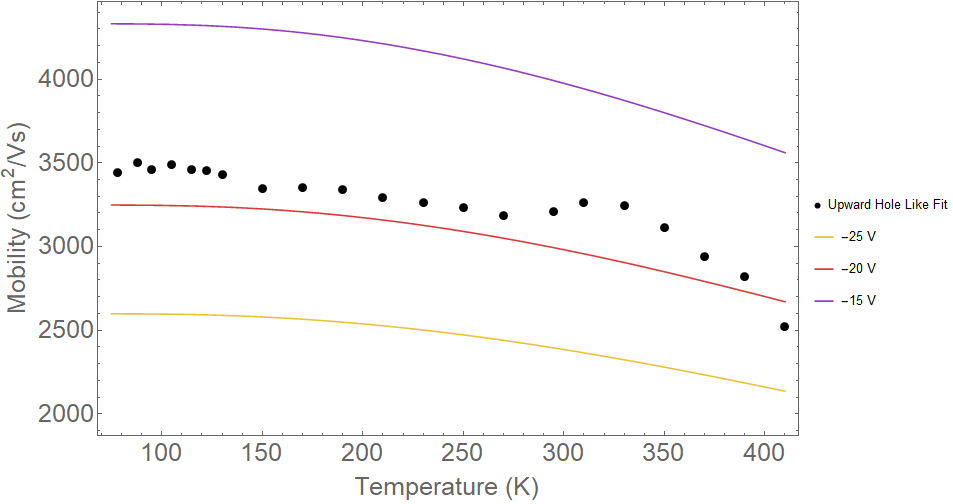
\includegraphics[width=\textwidth]{chap4/exf06/phonons/mobility}
	\caption[EXF06 temp. \& $V_g$ dependent mobility]{EXF06 temp. \& $V_g$ dependent mobility}\label{fig:exf06_mobility}
\end{figure}

%\begin{subfigure}[b]{0.5\textwidth}
%	\centering
%	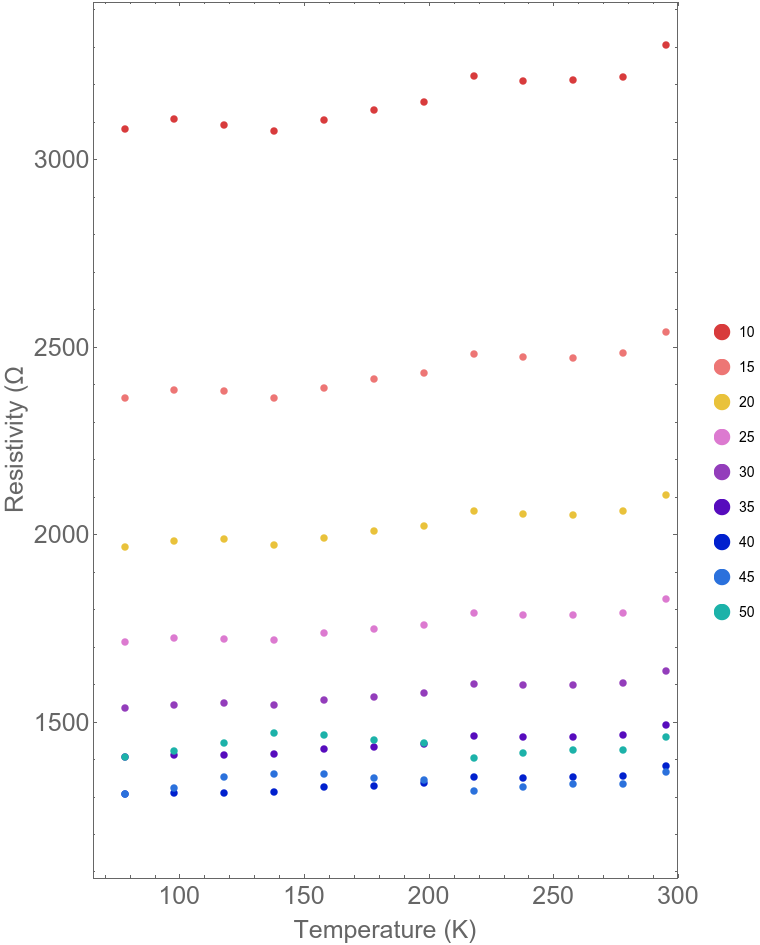
\includegraphics[width=\textwidth]{chap4/cvd01/CVD001_Res_vs_T_downward}
%	\caption[CVD01 temperature dependent conductivity]{Gate and temperature dependent conductivity of CVD01}\label{fig:cvd_temp_gate}
%\end{subfigure}

\subsection{hBN transfer}


\end{document}